

\chapter{数值结果验证}

\section{基准算例概述}

为了验证\ProgramName 程序的临界计算及时空动力学计算功能,
本章使用常用的三个不含热工反馈的时空动力学基准题对程序的结果进行验证。
临界计算的对比程序选用广泛使用的细网有限差分多群扩散程序——Citation。

\subsection{静态IAEA PWR三维基准问题}
\label{sec:result.test.iaea}

IAEA 三维压水堆基准题是三维两群扩散基准题,
由177个燃料组件构成,堆芯取$1/4$,
大小为170cm $\times$ 170cm $\times$ 380cm,
堆芯的几何结构见\floatref{fig:result.test.iaea},
堆芯中心为对称边界条件,外侧边界入流为0,外侧也可取等效边界条件\cite{center1977benchmark}
\begin{align}
  \frac{\partial \phi_g}{\partial n}=-\frac{0.4692}{D_g}\phi_g
\end{align}
各材料界面见\floatref{tab:result.test.iaea.mat},
裂变谱取$\chi_1=1$,$\chi_2=0$。

\begin{table}[h]
\centering
\caption{\label{tab:result.test.iaea.mat}静态IAEA PWR 三维基准题材料截面}
\begin{tabular}{cccccc}
\topline
材料 & 能群$g$ & $D_g/\mathrm{cm}$ & $\Sigma_{a,g}/\mathrm{cm}^{-1}$
    & $\nu\Sigma_{f,g}/n,\mathrm{cm}^{-1}$
    & $\Sigma_{s,1\rightarrow2}/\mathrm{cm}^{-1}$\\
\midline
\multirow{2}{*}{M1} 
  & 1 & 1.5 & 0.01 & 0 & \multirow{2}{*}{0.02} \\
  & 2 & 0.4 & 0.08 & 0.135 &\\
\multirow{2}{*}{M2} 
  & 1 & 1.5 & 0.01 & 0 & \multirow{2}{*}{0.02} \\
  & 2 & 0.4 & 0.085 & 0.135 &\\
\multirow{2}{*}{M3} 
  & 1 & 1.5 & 0.01 & 0 & \multirow{2}{*}{0.02} \\
  & 2 & 0.4 & 0.13 & 0.135 &\\
\multirow{2}{*}{M4} 
  & 1 & 2.0 & 0 & 0 & \multirow{2}{*}{0.04} \\
  & 2 & 0.3 & 0.01 & 0 &\\
\multirow{2}{*}{M5} 
  & 1 & 2.0 & 0 & 0 & \multirow{2}{*}{0.04} \\
  & 2 & 0.3 & 0.055 & 0 &\\
\bottomline
\end{tabular}
\end{table}

\begin{figure}
\centering
\begin{subfigure}{\textwidth}
\centering
\begin{tikzpicture}[scale=0.7, transform shape]
\def\lenscale{0.06}

\def\x#1{#1*\lenscale}
\def\zz#1{#1*\lenscale-8}
\def\z#1{#1*\lenscale}

\draw [very thick] (0,0) -- (\x{170},0) 
            -- (\x{170}, \zz{380}) -- (0, \zz{380});
\draw [loosely dashdotted] (0,0) -- (0, \zz{380});
\draw (0,\z{20}) -- (\x{150},\z{20}) -- (\x{150},\zz{360}) -- (0,\zz{360});
\draw (\x{10},\z{20}) -- (\x{10},\zz{380});
\draw [dashed] (\x{30},\zz{380}) -- (\x{30},\zz{280}) -- (\x{50},\zz{280}) -- (\x{50},\zz{380});
\draw (\x{70},\z{20}) -- (\x{70},\zz{380});
\draw (\x{90}, \z{20}) -- (\x{90},\zz{380});
\draw (\x{130},\z{20}) -- (\x{130},\zz{360});
\node at (\x{10},\z{80}) {\huge $\approx$};
\node at (\x{70},\z{80}) {\huge $\approx$};
\node at (\x{90},\z{80}) {\huge $\approx$};
\node at (\x{130},\z{80}) {\huge $\approx$};
\node at (\x{150},\z{80}) {\huge $\approx$};
\node at (\x{170},\z{80}) {\huge $\approx$};

\node [left] at (0,0) {\Large 0};
\node [left] at (0,\z{20}) {\Large 20};
\node [left] at (0,\zz{280}) {\Large 280};
\node [left] at (0,\zz{360}) {\Large 360};
\node [left] at (0,\zz{380}) {\Large 380};

\foreach \xp in {0, 10,30,50,70,90,130,150,170}
{
\node [above] at (\x{\xp},\zz{380}) {\Large \xp};
}

\node at (\x{160}, \zz{260}) {\Large M4};
\node at (\x{140}, \zz{260}) {\Large M1};
\node at (\x{110}, \zz{260}) {\Large M2};
\node at (\x{80}, \zz{260}) {\Large M3};
\node at (\x{40}, \zz{260}) {\Large M2};

\draw [-latex new, arrow head=3mm] (-1,\zz{260}) -- (\x{5}, \zz{260});
\node [left] at (-1, \zz{260}) {\Large M3};

%\draw [-latex new, arrow head=3mm] (-1,\zz{320}) -- (\x{40}, \zz{320});
%\node [left] at (-1, \zz{320}) {\Large Mp3};
\node at (\x{40}, \zz{320}) {\Large M3};

\node at (\x{80}, \zz{370}) {\Large M5};
\node at (\x{60}, \zz{370}) {\Large M4};
\node at (\x{40}, \zz{370}) {\Large M5};
\node at (\x{20}, \zz{370}) {\Large M4};

\draw [-latex new, arrow head=3mm] (-1,\zz{370}) -- (\x{5}, \zz{370});
\node [left] at (-1, \zz{370}) {\Large M5};

\node [above] at (-0.5,\zz{380}+0.5) {\Large cm};
\node [above] at (\x{170}+1,\zz{380}) {\Large cm};
\end{tikzpicture}
\caption{纵截面图}
\end{subfigure}
\begin{subfigure}{\textwidth}
\centering
\begin{tikzpicture}[scale=0.7, transform shape]
\def\lenscale{0.06}
\def\x#1{#1*\lenscale}

\draw [loosely dashdotted] (\x{170},0) -- (0,0) -- (0,\x{170});
%\draw [loosely dashdotted] (0,0) -- (\x{170},\x{170});

\draw (\x{10},0) -- (\x{10},\x{10}) -- (0,\x{10});

\draw (\x{70},0) -- (\x{70},\x{10}) -- (\x{90},\x{10}) -- (\x{90},0);
\draw (0,\x{70}) -- (\x{10},\x{70}) -- (\x{10},\x{90}) -- (0,\x{90});
\node [left] at (-1,\x{80}) {\Large M3};
\draw [-latex new, arrow head=3mm] (-1,\x{80}) -- (\x{5}, \x{80});
\node at (\x{80},\x{5}) {\Large M3};

\draw (\x{30},\x{30}) rectangle (\x{50},\x{50});
\node at (\x{40},\x{40}) {\Large M3};

\draw (0,\x{130}) -- (\x{30},\x{130}) -- (\x{30},\x{110})
           -- (\x{70},\x{110}) -- (\x{70},\x{70})
           -- (\x{110},\x{70}) -- (\x{110},\x{30})-- (\x{130},\x{30})
           -- (\x{130},0);
\node at (\x{40},\x{80}) {\Large M2};

\draw (\x{70},\x{70}) rectangle (\x{90},\x{90});
\node at (\x{80},\x{80}) {\Large M3};

\draw (0,\x{150}) -- (\x{50},\x{150}) -- (\x{50},\x{130})
           -- (\x{90},\x{130}) -- (\x{90},\x{110})
           -- (\x{110},\x{110})
           -- (\x{110},\x{90}) -- (\x{130},\x{90})-- (\x{130},\x{50})
           -- (\x{150},\x{50}) -- (\x{150},0);
\node at (\x{50},\x{120}) {\Large M1};

\draw [very thick] (0,\x{170}) -- (\x{70},\x{170}) -- (\x{70},\x{150})
           -- (\x{110},\x{150}) -- (\x{110},\x{130})
           -- (\x{130},\x{130})
           -- (\x{130},\x{110}) -- (\x{150},\x{110})-- (\x{150},\x{70})
           -- (\x{170},\x{70}) -- (\x{170},0);
\node at (\x{70},\x{140}) {\Large M4};

\foreach \xp in {0, 10,30,50,70,90,130,150,170}
{
\node [below] at (\x{\xp},0) {\Large \xp};
\node [left] at (0,\x{\xp}) {\Large \xp};
}

\node [below] at (\x{170}+1,0) {\Large cm};
\node [left] at (0, \x{170}+0.5) {\Large cm};

\draw [-latex new, arrow head=3mm](-1,\x{5}) -- (\x{5},\x{5});
\node [left] at (-1,\x{5}) {\Large M3};

\end{tikzpicture}
\caption{横截面图}
\end{subfigure}
\caption{\label{fig:result.test.iaea}静态IAEA PWR 三维基准题堆芯几何}
\end{figure}

\FloatBarrier
\subsection{动态TWIGL二维基准问题}
\label{sec:result.test.twigl}
TWIGL是二维两群扩散时空动力学基准题,
在1969年由Hageman和Yasinsky
于文献\onlinecite{hageman1969comparison}中提出,
堆芯取$1/4$,大小为80cm $\times$ 80cm,
堆芯的几何结构见\floatref{fig:result.test.twigl},
堆芯中心为对称边界条件,外侧边界入流为0。\cite{gehin1992quasi}

\begin{figure}[h]
\centering
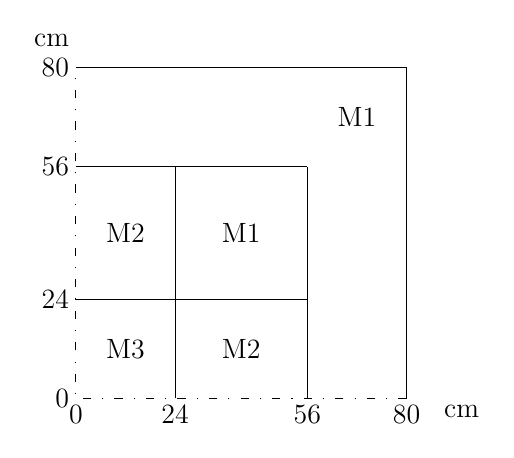
\begin{tikzpicture}[scale=0.7, transform shape]
\def\lenscale{0.075}
\def\x#1{#1*\lenscale}

\draw [loosely dashdotted] (\x{80},0) -- (0,0) -- (0,\x{80});

\draw (\x{24},0) -- (\x{24},\x{56});
\draw (0,\x{24}) -- (\x{56},\x{24});
\draw (\x{56},0) -- (\x{56},\x{56});
\draw (0,\x{56}) -- (\x{56},\x{56});
\draw (\x{80},0) -- (\x{80},\x{80});
\draw (0,\x{80}) -- (\x{80},\x{80});

\node at (\x{12},\x{12}) {\Large M3};
\node at (\x{40},\x{12}) {\Large M2};
\node at (\x{12},\x{40}) {\Large M2};
\node at (\x{40},\x{40}) {\Large M1};
\node at (\x{68},\x{68}) {\Large M1};

\foreach \xp in {0, 24, 56,80}
{
\node [below] at (\x{\xp},0) {\Large \xp};
\node [left] at (0,\x{\xp}) {\Large \xp};
}

\node [below] at (\x{80}+1,0) {\Large cm};
\node [left] at (0, \x{80}+0.5) {\Large cm};

\end{tikzpicture}
\caption{\label{fig:result.test.twigl}动态TWIGL二维基准题堆芯几何}
\end{figure}

各材料截面见\floatref{tab:result.test.twigl.mat},
裂变谱和缓发中子谱取$\chi_1=1$,$\chi_2=0$。
群速度为
\begin{align}
  v_1=1.0\times10^7\mathrm{cm/s} \qquad
  v_2=2.0\times10^5\mathrm{cm/s}
\end{align}
缓发中子为单组缓发中子
\begin{align}
  \beta=0.0075 \qquad
  \lambda=0.08\mathrm{s}^{-1}
\end{align}
反应性引入方式
\begin{enumerate}
\item 阶跃引入:
\begin{align}
\Delta\Sigma_{a,2}&=-0.0035\mathrm{cm}^{-1} \quad t=0
\end{align}

\item 线性引入:
\begin{align}
\Sigma_{a,2}(t)&=\begin{cases}
    (1-0.11667t)\Sigma_{a,2}(0) & t\le 0.2\\
    0.97666\Sigma_{a,2}(0) & t > 0.2
  \end{cases}
\end{align}
\end{enumerate}

\begin{table}
\centering
\caption{\label{tab:result.test.twigl.mat}动态TWIGL二维基准题材料截面}
\begin{tabular}{cccccc}
\topline
材料 & 能群$g$ & $D_g/\mathrm{cm}$ & $\Sigma_{a,g}/\mathrm{cm}^{-1}$
    & $\nu\Sigma_{f,g}/n,\mathrm{cm}^{-1}$
    & $\Sigma_{s,1\rightarrow2}/\mathrm{cm}^{-1}$\\
\midline
\multirow{2}{*}{M1} 
  & 1 & 1.4 & 0.01 & 0.007 & \multirow{2}{*}{0.01} \\
  & 2 & 0.4 & 0.15 & 0.2 &\\
\multirow{2}{*}{M2} 
  & 1 & 1.4 & 0.01 & 0.007 & \multirow{2}{*}{0.01} \\
  & 2 & 0.4 & 0.15 & 0.2 &\\
\multirow{2}{*}{M3} 
  & 1 & 1.3 & 0.008 & 0.003 & \multirow{2}{*}{0.01} \\
  & 2 & 0.5 & 0.05 & 0.06 &\\
\bottomline
\end{tabular}
\end{table}

\FloatBarrier
\subsection{动态LMW三维基准问题}

LMW(Langenbuch-Maurer-Werner)基准题是
三维两群扩散中子时空动力学基准题,
大小为$1/4$堆芯,几何尺寸110cm $\times$ 110cm $\times$ 200cm,
见\floatref{fig:result.test.lmw}。\cite{langenbuch1977coarse,gehin1992quasi}

\begin{figure}
\centering
\begin{subfigure}{.45\textwidth}
\hspace{-1.5cm}
\begin{tikzpicture}[scale=0.7, transform shape]
\def\lenscale{0.075}
\def\x#1{#1*\lenscale}

\draw [loosely dashdotted] (\x{110},0) -- (0,0) -- (0,\x{110});

\draw (\x{10},\x{0}) -- (\x{10},\x{10}) -- (\x{0},\x{10});
\draw (\x{50},\x{0}) -- (\x{50},\x{10}) -- (\x{70},\x{10}) -- (\x{70},\x{0});
\draw (\x{0},\x{50}) -- (\x{10},\x{50}) -- (\x{10},\x{70}) -- (\x{0},\x{70});
\node at (\x{30},\x{10}) {\Large M1};
\node at (\x{60},\x{5}) {\Large M2};
\node at (\x{5},\x{60}) {\Large M2};
\node at (\x{5},\x{5}) {\Large M2};

\draw (\x{30},\x{30}) rectangle (\x{50},\x{50});
\node at (\x{40},\x{40}) {\Large M2};

\draw (\x{70},\x{0}) -- (\x{70},\x{50}) -- (\x{50},\x{50})
      -- (\x{50},\x{70}) -- (\x{0},\x{70});
\node at (\x{60},\x{60}) {\Large M3};

\draw (\x{90},\x{0}) -- (\x{90},\x{70}) -- (\x{70},\x{70})
      -- (\x{70},\x{90}) -- (\x{0},\x{90});
\node at (\x{80},\x{80}) {\Large M4};

\draw (\x{110},\x{0}) -- (\x{110},\x{90}) -- (\x{90},\x{90})
      -- (\x{90},\x{110}) -- (\x{0},\x{110});

\foreach \xp in {0, 10,30,50,70,90,110}
{
\node [below] at (\x{\xp},0) {\Large \xp};
\node [left] at (0,\x{\xp}) {\Large \xp};
}

\node [below] at (\x{110}+1,0) {\Large cm};
\node [left] at (0, \x{110}+0.5) {\Large cm};

\draw [-latex new, arrow head=3mm] (-1.25,\x{50}) -- (\x{0},\x{60});
\draw [-latex new, arrow head=3mm] (-1.25,\x{50}) -- (\x{60},\x{10});
\node [left] at (-1.25,\x{50}) {\Large 第一组};

\draw [-latex new, arrow head=3mm] (-1.25,\x{20}) -- (\x{5},\x{10});
\draw [-latex new, arrow head=3mm] (-1.25,\x{20}) -- (\x{30},\x{40});
\node [left] at (-1.25,\x{20}) {\Large 第二组};

\end{tikzpicture}
\caption{横截面图}
\end{subfigure}
\\[1cm]
\begin{subfigure}{.45\textwidth}
\begin{tikzpicture}[scale=0.7, transform shape]
\def\lenscale{0.06}

\def\x#1{#1*\lenscale}
\def\zz#1{#1*\lenscale}
\def\z#1{#1*\lenscale}

\draw [very thick] (0,0) -- (\x{110},0) 
            -- (\x{110}, \zz{200}) -- (0, \zz{200});
\draw [loosely dashdotted] (0,0) -- (0, \zz{200});

\draw (0,\z{20}) -- (\x{90},\z{20}) -- (\x{90},\x{180}) -- (0,\zz{180});
\draw (\x{70},\x{20}) -- (\x{70},\x{180});

\node [left] at (0,0) {\Large 0};
\node [left] at (0,\z{20}) {\Large 20};
\node [left] at (0,\z{60}) {\Large 60};
\node [left] at (0,\z{100}) {\Large 100};
\node [left] at (0,\zz{180}) {\Large 180};
\node [left] at (0,\zz{200}) {\Large 200};

\node at (\x{30},\x{40}) {\Large M1};
\node at (\x{80},\x{100}) {\Large M3};
\node at (\x{100},\x{100}) {\Large M4};
\node at (\x{20},\x{190}) {\Large M4};
\node at (\x{40},\x{190}) {\Large M2};
\node at (\x{60},\x{190}) {\Large M2};
\draw [-latex new, arrow head=3mm] (-1,\x{190}) -- (\x{5},\x{190});
\node [left] at (-1,\x{190}) {\Large M2};

\draw [dashed] (\x{0},\x{100}) -- (\x{10},\x{100}) -- (\x{10},\x{200});
\draw (\x{10},\x{180}) -- (\x{10},\x{200});
\draw (\x{50},\x{200}) -- (\x{50},\x{100}) -- (\x{70},\x{100}) -- (\x{70},\x{200});
\draw [dashed] (\x{30},\x{180}) -- (\x{30},\x{200});

\node at (\x{60},\x{140}) {\Large M2};
\draw [-latex new, arrow head=3mm] (-1,\x{140}) -- (\x{5},\x{140});
\node [left] at (-1,\x{140}) {\Large M2};

\draw [-latex new, arrow head=3mm] (-1,\x{70}) -- (\x{5},\x{100});
\draw [-latex new, arrow head=3mm] (-1,\x{70}) -- (\x{60},\x{100});
\node [left] at (-1,\x{70}) {\Large 第一组};
\draw [-latex new, arrow head=3mm] (-1,\x{160}) -- (\x{5},\x{180});
\draw [-latex new, arrow head=3mm] (-1,\x{160}) -- (\x{40},\x{180});
\node [left] at (-1,\x{160}) {\Large 第二组};

\foreach \xp in {0,10,30,50,70,90,110}
{
\node [above] at (\x{\xp},\zz{200}) {\Large \xp};
}

\node at (-0.75,\zz{200}+0.75) {\Large cm};
\end{tikzpicture}
\caption{纵截面图(初始时控制棒位置)}
\end{subfigure}
\begin{subfigure}{.45\textwidth}
\begin{tikzpicture}[scale=0.7, transform shape]
\def\lenscale{0.06}

\def\x#1{#1*\lenscale}
\def\zz#1{#1*\lenscale}
\def\z#1{#1*\lenscale}

\draw [very thick] (0,0) -- (\x{110},0) 
            -- (\x{110}, \zz{200}) -- (0, \zz{200});
\draw [loosely dashdotted] (0,0) -- (0, \zz{200});

\draw (0,\z{20}) -- (\x{90},\z{20}) -- (\x{90},\x{180}) -- (0,\zz{180});
\draw (\x{70},\x{20}) -- (\x{70},\x{180});

\node [left] at (0,0) {\Large 0};
\node [left] at (0,\z{20}) {\Large 20};
\node [left] at (0,\z{60}) {\Large 60};
\node [left] at (0,\z{100}) {\Large 100};
\node [left] at (0,\zz{180}) {\Large 180};
\node [left] at (0,\zz{200}) {\Large 200};

\node at (\x{30},\x{40}) {\Large M1};
\node at (\x{80},\x{100}) {\Large M3};
\node at (\x{100},\x{100}) {\Large M4};
\node at (\x{20},\x{190}) {\Large M4};
\node at (\x{40},\x{190}) {\Large M2};
\node at (\x{60},\x{190}) {\Large M2};
\draw [-latex new, arrow head=3mm] (-1,\x{190}) -- (\x{5},\x{190});
\node [left] at (-1,\x{190}) {\Large M2};

\draw (\x{0},\x{60}) -- (\x{10},\x{60}) -- (\x{10},\x{200});
\draw [dashed] (\x{30},\x{200}) -- (\x{30},\x{60}) -- (\x{50},\x{60}) -- (\x{50},\x{200});
\draw (\x{50},\x{180}) -- (\x{50},\x{200});
\draw (\x{70},\x{180}) -- (\x{70},\x{200});

\draw [-latex new, arrow head=3mm] (-1,\x{30}) -- (\x{5},\x{60});
\draw [-latex new, arrow head=3mm] (-1,\x{30}) -- (\x{40},\x{60});
\node [left] at (-1,\x{30}) {\Large 第二组};
\draw [-latex new, arrow head=3mm] (-1,\x{160}) -- (\x{5},\x{180});
\draw [-latex new, arrow head=3mm] (-1,\x{160}) -- (\x{60},\x{180});
\node [left] at (-1,\x{160}) {\Large 第一组};

\node at (\x{40},\x{120}) {\Large M2};
\draw [-latex new, arrow head=3mm] (-1,\x{120}) -- (\x{5},\x{120});
\node [left] at (-1,\x{120}) {\Large M2};

\foreach \xp in {0,10,30,50,70,90,110}
{
\node [above] at (\x{\xp},\zz{200}) {\Large \xp};
}

\node at (-0.75,\zz{200}+0.75) {\Large cm};
\end{tikzpicture}
\caption{纵截面图(最终控制棒位置)}
\end{subfigure}
\caption{\label{fig:result.test.lmw}动态LMW三维基准题堆芯几何}
\end{figure}

\begin{table}
\centering
\caption{\label{tab:result.test.lmw.mat}动态LMW三维基准题材料截面}
\begin{tabular}{cccccc}
\topline
材料 & 能群$g$ & $D_g/\mathrm{cm}$ & $\Sigma_{a,g}/\mathrm{cm}^{-1}$
    & $\nu\Sigma_{f,g}/n,\mathrm{cm}^{-1}$
    & $\Sigma_{s,1\rightarrow2}/\mathrm{cm}^{-1}$\\
\midline
\multirow{2}{*}{M1} 
  & 1 & 1.423913 & 0.01040206 & 0.006477691 & \multirow{2}{*}{0.0175555} \\
  & 2 & 0.356306 & 0.08766217 & 0.1127328 &\\
\multirow{2}{*}{M2} 
  & 1 & 1.423913 & 0.01095206 & 0.006477691 & \multirow{2}{*}{0.0175555} \\
  & 2 & 0.356306 & 0.09146217 & 0.1127328 &\\
\multirow{2}{*}{M3} 
  & 1 & 1.425611 & 0.01099263 & 0.007503284 & \multirow{2}{*}{0.01717768} \\
  & 2 & 0.350574 & 0.09925634 & 0.1378004 &\\
\multirow{2}{*}{M4} 
  & 1 & 1.634227 & 0.002660573 & 0 & \multirow{2}{*}{0.02759693} \\
  & 2 & 0.264002 & 0.04936351 & 0 &\\
\bottomline
\end{tabular}
\end{table}


算例包含两组控制棒,开始时第一组控制棒以3cm/s的速度拔出,
26.67s时停止。第二组控制棒从7.5s开始以同样的速度插入,47.5s时停止,
控制棒位置随时间变化见\floatref{fig:result.test.lmw.rob}。
\begin{figure}
\centering
\includegraphics[scale=0.9]{result-test-lmw-rob}
\caption{\label{fig:result.test.lmw.rob}LMW算例控制棒位置随时间变化图}
\end{figure}

裂变谱和缓发中子谱取$\chi_1=1$,$\chi_2=0$。
群速度为
\begin{align}
  \left\{
  \begin{aligned}
  v_1&=1.25\times10^7\mathrm{cm/s}\\
  v_2&=2.5\times10^5\mathrm{cm/s}
  \end{aligned}
  \right.
\end{align}
缓发中子有6组,见\floatref{tab:result.test.lmw.mat.c}。

\begin{table}
\centering
\caption{\label{tab:result.test.lmw.mat.c}动态LMW三维基准题缓发中子数据}
\begin{tabular}{ccc}
\topline
缓发中子组 & 缓发中子份额$\beta_i$ & 衰变常数$\lambda_i/\mathrm{s}^{-1}$\\
\midline
1 & 0.000247 & 0.0127\\
2 & 0.0013845 & 0.0317\\
3 & 0.001222 & 0.1150\\
4 & 0.0026455 & 0.3110\\
5 & 0.000832 & 1.400\\
6 & 0.000169 & 3.870\\
\bottomline
\end{tabular}
\end{table}


\section{数值结果验证}

在比较\ProgramName 的计算结果和参考结果之前,
先介绍本文使用的通量结果偏差的计算方式。

对于临界问题,程序计算得到的通量分布结果的绝对值无意义,
有意义的是各网格上通量的相对大小关系,
所以一般都需要对结果进行归一化,
再比较归一化后的通量结果。
那么选择的归一化方法就会影响到计算结果的对比,
常见的归一化方式是总功率归一化和最大通量归一化,
但这两种方法都有各自的问题:
由于堆芯中通量分布在不同的网格上可相差数个量级,
如果按照堆芯总功率进行归一化,那么堆芯中部功率较高的部分对归一化系数影响很大,
高通量区域的误差会通过归一化系数转移到到低通量区域上;
同理使用最大通量归一化时,通量最高处的误差会影响到其他所有点的误差结果。
在常见的组件级通量统计中,这种问题并不明显,
但在细网结果的相对误差比较中,这种影响就被放大了。

为了减小高通量网格对归一化系数的影响,本文使用所有网格上的相对幅值的均值作为
归一化系数,即待验证的通量分布$\phi$和参考通量分布$\psi$间的相对归一化系数取为
\begin{align}
  \eta = \frac{\ \displaystyle\sum_{\bm{k},g}\frac{\phi_{\bm{k},g}}{\psi_{\bm{k},g}}\ }
              {\displaystyle\sum_{\bm{k},g}1}
\end{align}
其中$\bm{k}$为空间网格编号,
则归一化后的各网格的最大相对误差为
\begin{align}
  e_\mathrm{max} = \max_{\bm{k},g}
      \left|
        \frac{\phi_{\bm{k},g}}{\eta\cdot\psi_{\bm{k},g}} - 1
      \right|
\end{align}
本文以后提到的最大相对误差均是指上式所定义的最大相对误差,
而且为了更好地反映有实际意义的堆芯内的通量的相对误差,
一般把堆芯活性区以外的水反射层处通量极低的网格滤掉。

本文中如无特殊声明,计算环境均为
\begin{itemize}
\item CPU: 2$\times$ Intel Xeon CPU X5670 2.93GHz (双路服务器)
\item 内存:24GB
\item GPU:NVIDIA GeForce GTX TITAN,6GB显存
\item 操作系统:Windows 7 SP1 64位
\end{itemize}

\subsection{静态IAEA PWR三维基准题}

使用Citation的计算结果作为参考解,
通量收敛精度$\epsilon_\phi$取$5\times10^{-7}$,
对于5cm、2.5cm、2cm、1cm的$k_\mathrm{eff}$计算结果
见\floatref{tab:result.iaea.citation}。
\ProgramName 的通量收敛精度取$\epsilon'_\phi=10^{-6}$,
需要注意的是\ProgramName 和Citation的收敛精度计算方式不同,
计算结果见\floatref{tab:result.iaea.self},
其中$\max\epsilon_{\phi_{A,g}}$表示各组件通量的最大相对误差。

可见在该精度下\ProgramName 计算的$k_\mathrm{eff}$ 偏差小于$1\times10^{-5}$,
细网通量最大相对误差小于$10^{-3}$,
对于Multilevel方法通量最大相对误差小于$9\times10^{-4}$。
1cm网格$1/8$堆芯的组件通量相对偏差结果见\floatref{fig:result.iaea.aphitable.cg}及
\floatref{fig:result.iaea.aphitable.cgml},
其中$\phi_R$是\ProgramName 的计算结果,$\phi_C$是Citation的计算结果,
$\epsilon(\phi)$是两者的相对偏差。

\begin{table}[h]
\centering
\caption{静态IAEA PWR三维基准题Citation计算结果}
\label{tab:result.iaea.citation}
\begin{tabular}{ccr}
\topline
网格尺寸/cm & $k_\mathrm{eff}$ & 计算时间/s \\
\midline
5.0 & 1.0288101 &    6.36 \\
2.5 & 1.0290707 &  233.70 \\
2.0 & 1.0291338 &  856.08 \\
1.0 & 1.0292318 & 38005.0 \\
\bottomline
\end{tabular}
\end{table}

\begin{table}
\centering
\caption{静态IAEA PWR三维基准题\ProgramName 计算结果及误差}
\label{tab:result.iaea.self}
\subcaptionbox{CG-SG算法\label{tab:result.iaea.self.cg}}{
\begin{tabular}{crcccc}
\topline
网格尺寸/cm 
        & 计算时间/s & $k_\mathrm{eff}$ 
        & $\epsilon_{k_\mathrm{eff}}$
        & $\max\epsilon_{\phi_{\bm{k},g}}$
        & $\max\epsilon_{\phi_{A,g}}$\\
\midline
5.0 &    2.637 & 1.0288103 & $1.9\times10^{-7}$ & $5.7\times10^{-4}$ & $1.6\times10^{-5}$\\
2.5 &    8.268 & 1.0290725 & $1.8\times10^{-6}$ & $5.8\times10^{-4}$ & $8.3\times10^{-6}$\\
2.0 &   15.444 & 1.0291343 & $4.9\times10^{-7}$ & $5.9\times10^{-4}$ & $7.5\times10^{-6}$\\
1.0 &  164.877 & 1.0292398 & $8.0\times10^{-6}$ & $1.0\times10^{-3}$ & $6.0\times10^{-5}$\\
\bottomline
\end{tabular}
}
\\[1cm]
\subcaptionbox{CG-SG Multilevel算法\label{tab:result.iaea.self.cgml}}{
\begin{tabular}{crcccc}
\topline
网格尺寸/cm 
        & 计算时间/s & $k_\mathrm{eff}$ 
        & $\epsilon_{k_\mathrm{eff}}$
        & $\max\epsilon_{\phi_{\bm{k},g}}$
        & $\max\epsilon_{\phi_{A,g}}$\\
\midline
2.5 &    6.006 & 1.0290727 & $2.0\times10^{-6}$ & $6.3\times10^{-4}$ & $3.5\times10^{-5}$\\
1.0 &   78.749 & 1.0292401 & $8.2\times10^{-6}$ & $8.8\times10^{-4}$ & $4.2\times10^{-5}$\\
\bottomline
\end{tabular}
}
\end{table}


\begin{figure}
\centering
\subcaptionbox{快群}{
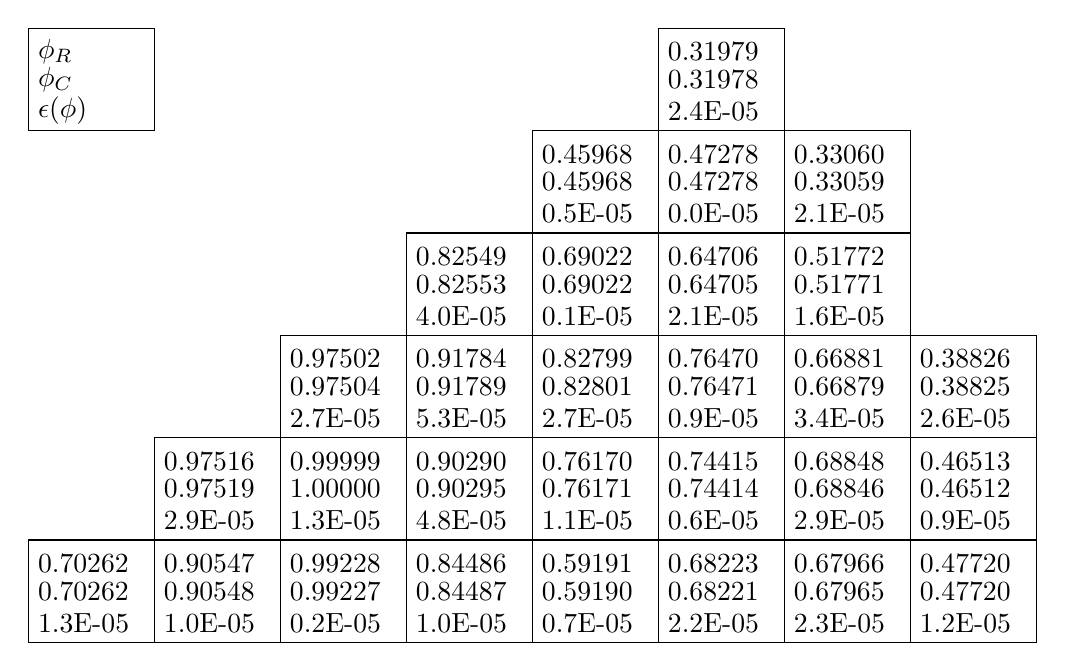
\begin{tikzpicture}
\def\di#1#2#3#4#5{
\def\boxx{1.6}
\def\boxy{1.3}
\draw (#1*\boxx, #2*\boxy) -- +(\boxx,0) -- +(\boxx,\boxy) -- +(0,\boxy) -- +(0,0);
\node [right] at (#1*\boxx,#2*\boxy+1) {#3};
\node [right]  at (#1*\boxx,#2*\boxy+0.65) {#4};
\node [right]  at (#1*\boxx,#2*\boxy+0.25) {#5};
}
\di{0}{5}{$\phi_R$}{$\phi_C$}{$\epsilon(\phi)$}
\di{0}{0}{0.70262}{0.70262}{1.3E-05}
\di{1}{0}{0.90547}{0.90548}{1.0E-05}
\di{1}{1}{0.97516}{0.97519}{2.9E-05}
\di{2}{0}{0.99228}{0.99227}{0.2E-05}
\di{2}{1}{0.99999}{1.00000}{1.3E-05}
\di{2}{2}{0.97502}{0.97504}{2.7E-05}
\di{3}{0}{0.84486}{0.84487}{1.0E-05}
\di{3}{1}{0.90290}{0.90295}{4.8E-05}
\di{3}{2}{0.91784}{0.91789}{5.3E-05}
\di{3}{3}{0.82549}{0.82553}{4.0E-05}
\di{4}{0}{0.59191}{0.59190}{0.7E-05}
\di{4}{1}{0.76170}{0.76171}{1.1E-05}
\di{4}{2}{0.82799}{0.82801}{2.7E-05}
\di{4}{3}{0.69022}{0.69022}{0.1E-05}
\di{4}{4}{0.45968}{0.45968}{0.5E-05}
\di{5}{0}{0.68223}{0.68221}{2.2E-05}
\di{5}{1}{0.74415}{0.74414}{0.6E-05}
\di{5}{2}{0.76470}{0.76471}{0.9E-05}
\di{5}{3}{0.64706}{0.64705}{2.1E-05}
\di{5}{4}{0.47278}{0.47278}{0.0E-05}
\di{5}{5}{0.31979}{0.31978}{2.4E-05}
\di{6}{0}{0.67966}{0.67965}{2.3E-05}
\di{6}{1}{0.68848}{0.68846}{2.9E-05}
\di{6}{2}{0.66881}{0.66879}{3.4E-05}
\di{6}{3}{0.51772}{0.51771}{1.6E-05}
\di{6}{4}{0.33060}{0.33059}{2.1E-05}
\di{7}{0}{0.47720}{0.47720}{1.2E-05}
\di{7}{1}{0.46513}{0.46512}{0.9E-05}
\di{7}{2}{0.38826}{0.38825}{2.6E-05}
\end{tikzpicture}
}

\subcaptionbox{热群}{
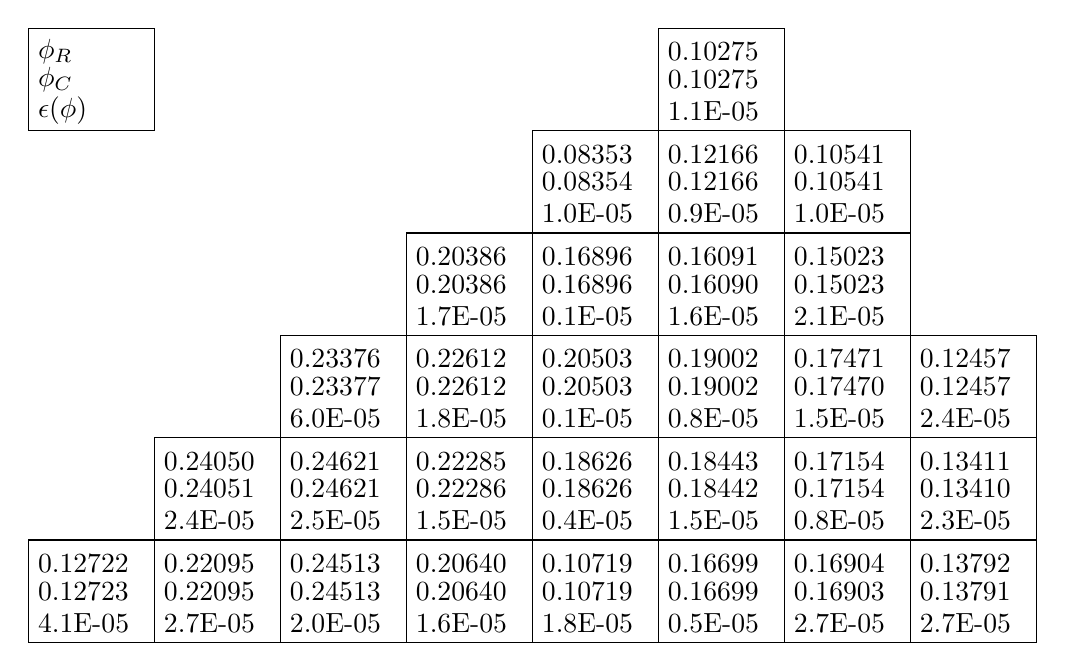
\begin{tikzpicture}
\def\di#1#2#3#4#5{
\def\boxx{1.6}
\def\boxy{1.3}
\draw (#1*\boxx, #2*\boxy) -- +(\boxx,0) -- +(\boxx,\boxy) -- +(0,\boxy) -- +(0,0);
\node [right] at (#1*\boxx,#2*\boxy+1) {#3};
\node [right]  at (#1*\boxx,#2*\boxy+0.65) {#4};
\node [right]  at (#1*\boxx,#2*\boxy+0.25) {#5};
}
\di{0}{5}{$\phi_R$}{$\phi_C$}{$\epsilon(\phi)$}
\di{0}{0}{0.12722}{0.12723}{4.1E-05}
\di{1}{0}{0.22095}{0.22095}{2.7E-05}
\di{1}{1}{0.24050}{0.24051}{2.4E-05}
\di{2}{0}{0.24513}{0.24513}{2.0E-05}
\di{2}{1}{0.24621}{0.24621}{2.5E-05}
\di{2}{2}{0.23376}{0.23377}{6.0E-05}
\di{3}{0}{0.20640}{0.20640}{1.6E-05}
\di{3}{1}{0.22285}{0.22286}{1.5E-05}
\di{3}{2}{0.22612}{0.22612}{1.8E-05}
\di{3}{3}{0.20386}{0.20386}{1.7E-05}
\di{4}{0}{0.10719}{0.10719}{1.8E-05}
\di{4}{1}{0.18626}{0.18626}{0.4E-05}
\di{4}{2}{0.20503}{0.20503}{0.1E-05}
\di{4}{3}{0.16896}{0.16896}{0.1E-05}
\di{4}{4}{0.08353}{0.08354}{1.0E-05}
\di{5}{0}{0.16699}{0.16699}{0.5E-05}
\di{5}{1}{0.18443}{0.18442}{1.5E-05}
\di{5}{2}{0.19002}{0.19002}{0.8E-05}
\di{5}{3}{0.16091}{0.16090}{1.6E-05}
\di{5}{4}{0.12166}{0.12166}{0.9E-05}
\di{5}{5}{0.10275}{0.10275}{1.1E-05}
\di{6}{0}{0.16904}{0.16903}{2.7E-05}
\di{6}{1}{0.17154}{0.17154}{0.8E-05}
\di{6}{2}{0.17471}{0.17470}{1.5E-05}
\di{6}{3}{0.15023}{0.15023}{2.1E-05}
\di{6}{4}{0.10541}{0.10541}{1.0E-05}
\di{7}{0}{0.13792}{0.13791}{2.7E-05}
\di{7}{1}{0.13411}{0.13410}{2.3E-05}
\di{7}{2}{0.12457}{0.12457}{2.4E-05}
\end{tikzpicture}
}
\caption{静态IAEA三维基准题\ProgramName 程序 CG-SG 1cm网格$1/8$堆芯组件通量相对偏差}
\label{fig:result.iaea.aphitable.cg}
\end{figure}


\begin{figure}
\centering
\subcaptionbox{快群}{
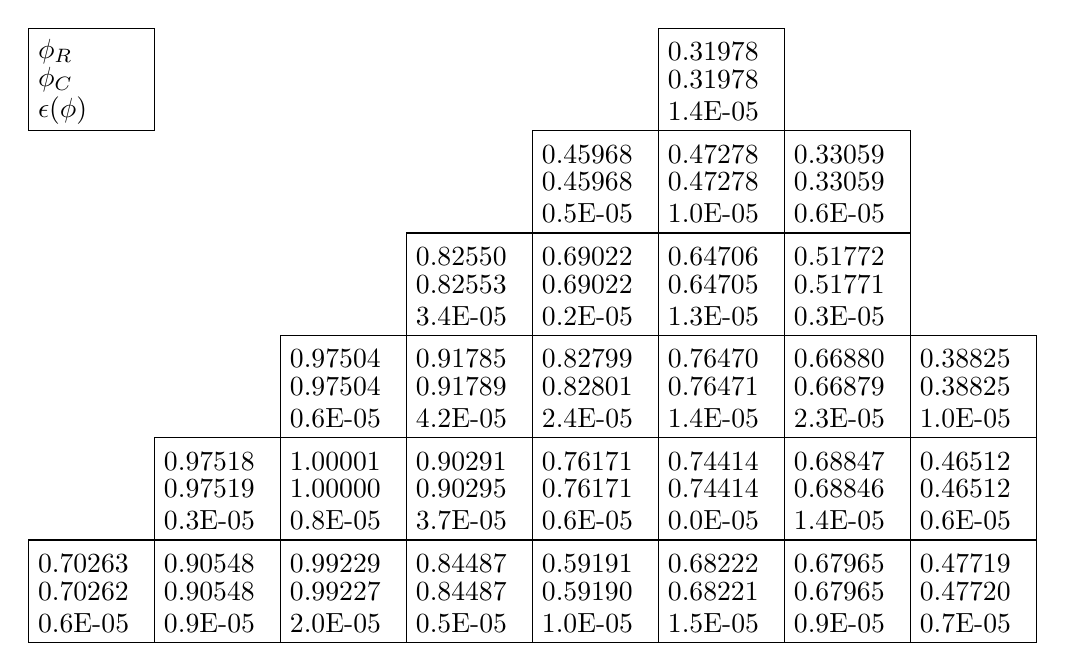
\begin{tikzpicture}
\def\di#1#2#3#4#5{
\def\boxx{1.6}
\def\boxy{1.3}
\draw (#1*\boxx, #2*\boxy) -- +(\boxx,0) -- +(\boxx,\boxy) -- +(0,\boxy) -- +(0,0);
\node [right] at (#1*\boxx,#2*\boxy+1) {#3};
\node [right]  at (#1*\boxx,#2*\boxy+0.65) {#4};
\node [right]  at (#1*\boxx,#2*\boxy+0.25) {#5};
}
\di{0}{5}{$\phi_R$}{$\phi_C$}{$\epsilon(\phi)$}
\di{0}{0}{0.70263}{0.70262}{0.6E-05}
\di{1}{0}{0.90548}{0.90548}{0.9E-05}
\di{1}{1}{0.97518}{0.97519}{0.3E-05}
\di{2}{0}{0.99229}{0.99227}{2.0E-05}
\di{2}{1}{1.00001}{1.00000}{0.8E-05}
\di{2}{2}{0.97504}{0.97504}{0.6E-05}
\di{3}{0}{0.84487}{0.84487}{0.5E-05}
\di{3}{1}{0.90291}{0.90295}{3.7E-05}
\di{3}{2}{0.91785}{0.91789}{4.2E-05}
\di{3}{3}{0.82550}{0.82553}{3.4E-05}
\di{4}{0}{0.59191}{0.59190}{1.0E-05}
\di{4}{1}{0.76171}{0.76171}{0.6E-05}
\di{4}{2}{0.82799}{0.82801}{2.4E-05}
\di{4}{3}{0.69022}{0.69022}{0.2E-05}
\di{4}{4}{0.45968}{0.45968}{0.5E-05}
\di{5}{0}{0.68222}{0.68221}{1.5E-05}
\di{5}{1}{0.74414}{0.74414}{0.0E-05}
\di{5}{2}{0.76470}{0.76471}{1.4E-05}
\di{5}{3}{0.64706}{0.64705}{1.3E-05}
\di{5}{4}{0.47278}{0.47278}{1.0E-05}
\di{5}{5}{0.31978}{0.31978}{1.4E-05}
\di{6}{0}{0.67965}{0.67965}{0.9E-05}
\di{6}{1}{0.68847}{0.68846}{1.4E-05}
\di{6}{2}{0.66880}{0.66879}{2.3E-05}
\di{6}{3}{0.51772}{0.51771}{0.3E-05}
\di{6}{4}{0.33059}{0.33059}{0.6E-05}
\di{7}{0}{0.47719}{0.47720}{0.7E-05}
\di{7}{1}{0.46512}{0.46512}{0.6E-05}
\di{7}{2}{0.38825}{0.38825}{1.0E-05}
\end{tikzpicture}
}

\subcaptionbox{热群}{
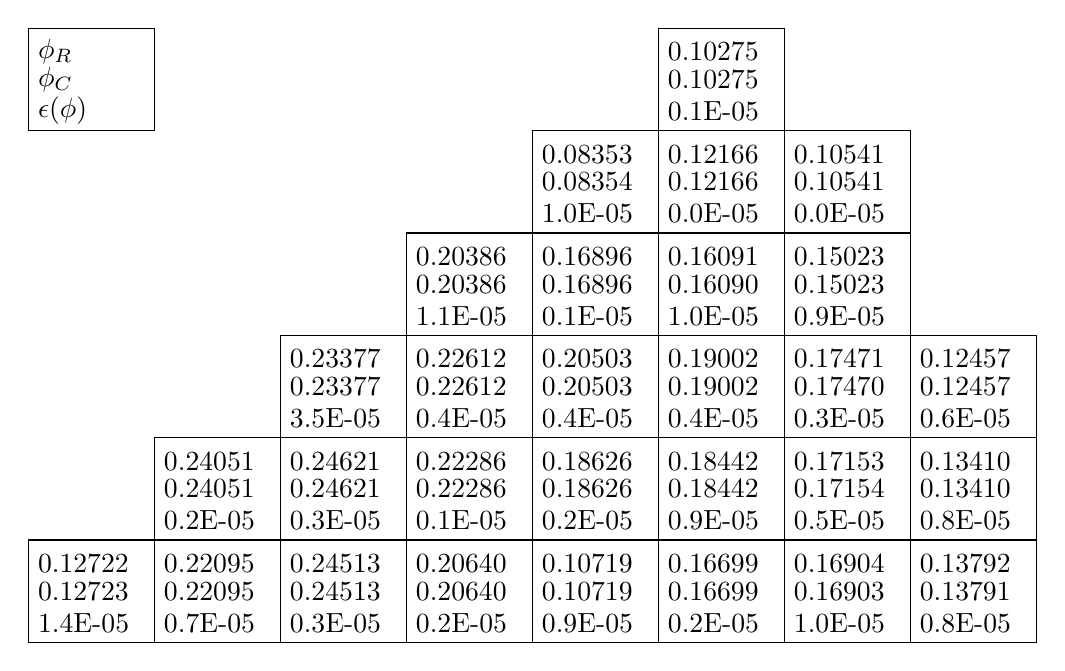
\begin{tikzpicture}
\def\di#1#2#3#4#5{
\def\boxx{1.6}
\def\boxy{1.3}
\draw (#1*\boxx, #2*\boxy) -- +(\boxx,0) -- +(\boxx,\boxy) -- +(0,\boxy) -- +(0,0);
\node [right] at (#1*\boxx,#2*\boxy+1) {#3};
\node [right]  at (#1*\boxx,#2*\boxy+0.65) {#4};
\node [right]  at (#1*\boxx,#2*\boxy+0.25) {#5};
}
\di{0}{5}{$\phi_R$}{$\phi_C$}{$\epsilon(\phi)$}
\di{0}{0}{0.12722}{0.12723}{1.4E-05}
\di{1}{0}{0.22095}{0.22095}{0.7E-05}
\di{1}{1}{0.24051}{0.24051}{0.2E-05}
\di{2}{0}{0.24513}{0.24513}{0.3E-05}
\di{2}{1}{0.24621}{0.24621}{0.3E-05}
\di{2}{2}{0.23377}{0.23377}{3.5E-05}
\di{3}{0}{0.20640}{0.20640}{0.2E-05}
\di{3}{1}{0.22286}{0.22286}{0.1E-05}
\di{3}{2}{0.22612}{0.22612}{0.4E-05}
\di{3}{3}{0.20386}{0.20386}{1.1E-05}
\di{4}{0}{0.10719}{0.10719}{0.9E-05}
\di{4}{1}{0.18626}{0.18626}{0.2E-05}
\di{4}{2}{0.20503}{0.20503}{0.4E-05}
\di{4}{3}{0.16896}{0.16896}{0.1E-05}
\di{4}{4}{0.08353}{0.08354}{1.0E-05}
\di{5}{0}{0.16699}{0.16699}{0.2E-05}
\di{5}{1}{0.18442}{0.18442}{0.9E-05}
\di{5}{2}{0.19002}{0.19002}{0.4E-05}
\di{5}{3}{0.16091}{0.16090}{1.0E-05}
\di{5}{4}{0.12166}{0.12166}{0.0E-05}
\di{5}{5}{0.10275}{0.10275}{0.1E-05}
\di{6}{0}{0.16904}{0.16903}{1.0E-05}
\di{6}{1}{0.17153}{0.17154}{0.5E-05}
\di{6}{2}{0.17471}{0.17470}{0.3E-05}
\di{6}{3}{0.15023}{0.15023}{0.9E-05}
\di{6}{4}{0.10541}{0.10541}{0.0E-05}
\di{7}{0}{0.13792}{0.13791}{0.8E-05}
\di{7}{1}{0.13410}{0.13410}{0.8E-05}
\di{7}{2}{0.12457}{0.12457}{0.6E-05}
\end{tikzpicture}
}
\caption{静态IAEA三维基准题\ProgramName 程序 CG-SG Multilevel 1cm网格$1/8$堆芯组件通量相对偏差}
\label{fig:result.iaea.aphitable.cgml}
\end{figure}

\subsection{动态TWIGL二维基准问题}

动态TWIGL二维基准题的计算结果及对比见\floatref{tab:result.twigl.power-compare.1}
和\floatref{tab:result.twigl.power-compare.2}。

\begin{table}[H]
\centering
\begin{minipage}{0.9\textwidth}
\centering
\caption{动态TWIGL二维基准问题(阶跃反应性)计算结果(堆芯相对功率)\label{tab:result.twigl.power-compare.1}}
\begin{tabular}{cccccc}
\topline
系统时刻/s & QUANDRY\footnote{使用解析节块法,时间步长0.01s,
             数据来源\onlinecite{smith1979analytic,zhaowenbo}。}
         & NEM\footnote{使用节块展开法,网格8cm$\times$8cm,时间步长0.005s,
             数据来源\onlinecite{bandini1990three,zhaowenbo}。}
         & NGFMN-K\footnote{使用节块格林函数法,网格8cm$\times$8cm,计算方法DIRK(5,4)-E,
             计算精度1e-5,数据来源\onlinecite{zhaowenbo}。}
         & SPANDEX\footnote{使用变时间步节块展开法,网格4cm$\times$4cm,时间步长0.0001s,
             数据来源\onlinecite{aviles1993development,sutton1996diffusion}。}
         & \ProgramName \footnote{本文工作,细网有限差分法,
             网格划分1cm$\times$1cm,时间步长$0.01$s。}
         \\
\midline
0.1 & 2.064 & 2.060 & 2.061 & 2.062 & 2.060 \\
0.2 & 2.076 & 2.078 & 2.079 & 2.079 & 2.079 \\
0.3 & 2.095 & 2.095 & 2.096 & 2.096 & 2.096 \\
0.4 & 2.112 & 2.113 & 2.114 & 2.114 & 2.114 \\
0.5 & 2.130 & 2.131 & 2.131 & 2.131 & 2.131 \\
\bottomline
\end{tabular}
\end{minipage}
\end{table}

\begin{table}[H]
\centering
\begin{minipage}{0.9\textwidth}
\centering
\caption{动态TWIGL二维基准问题(线性反应性)计算结果(堆芯相对功率)\label{tab:result.twigl.power-compare.2}}
\begin{tabular}{cccccc}
\topline
系统时刻/s & QUANDRY\footnote{时间步长0.005s,
             数据来源\onlinecite{smith1979analytic,zhaowenbo}。}
         & NEM\footnote{网格8cm$\times$8cm,时间步长0.005s,
             数据来源\onlinecite{bandini1990three,zhaowenbo}。}
         & NGFMN-K\footnote{网格8cm$\times$8cm,计算方法DIRK(5,4)-E,
             计算精度1e-5,数据来源\onlinecite{zhaowenbo}。}
         & SPANDEX\footnote{网格4cm$\times$4cm,时间步长0.0001s,
             数据来源\onlinecite{aviles1993development,sutton1996diffusion}。}
         & \ProgramName \footnote{网格划分1cm$\times$1cm,时间步长$0.005$s。}
         \\
\midline
0.1 & 1.305 & 1.309 & 1.309 & 1.309 & 1.309 \\
0.2 & 1.954 & 1.962 & 1.960 & 1.960 & 1.962 \\
0.3 & 2.074 & 2.075 & 2.075 & 2.075 & 2.076 \\
0.4 & 2.092 & 2.092 & 2.092 & 2.092 & 2.093 \\
0.5 & 2.109 & 2.110 & 2.110 & 2.110 & 2.111 \\
\bottomline
\end{tabular}
\end{minipage}
\end{table}

可见\ProgramName 和各种节块程序的结果符合的较好。


\subsection{动态LMW三维基准问题}

动态LMW三维基准题的计算结果及对比见\floatref{tab:result.lmw.power-compare}。

\begin{table}[H]
\begin{minipage}{\textwidth}
\centering
\caption{动态LMW三维基准问题计算结果(堆芯相对功率)}
\label{tab:result.lmw.power-compare}
\begin{tabular}{ccccccc}
\topline
\begin{tabular}{cc} 系统 \\ 时刻/s \end{tabular}
 & {\footnotesize SKETCH-N}\footnote{使用基于非线性迭代策略的CMFD方法,网格10cm$\times$10cm$\times$5cm,时间步长0.25s,
             数据来源\onlinecite{zimin1998nodal}。}
 & {\footnotesize PANTHER}\footnote{使用基于非线性迭代策略的解析节块法,网格10cm$\times$10cm$\times$5cm,时间步长0.25s,
             数据来源\onlinecite{sutton1996diffusion}。}
 & {\footnotesize NGFMN-K}\footnote{使用节块格林函数法,网格10cm$\times$10cm$\times$5cm,计算方法DIRK(5,4)-E,
             计算精度1e-5,数据来源\onlinecite{zhaowenbo}。}
 & {\footnotesize SPANDEX}\footnote{使用变时间步节块展开法,网格5cm$\times$5cm$\times$2.5cm,计算精度5e-2,
             数据来源\onlinecite{aviles1993development,sutton1996diffusion}。}
 & {\footnotesize NLSANMT}\footnote{使用基于非线性迭代策略的CMFD方法,网格10cm$\times$10cm$\times$5cm,时间步长0.25s,
             数据来源\onlinecite{liaochengkui,zhaowenbo}。}
 & {\footnotesize \ProgramName}\footnote{本文工作,细网有限差分法,
             网格划分1cm$\times$1cm$\times$1cm,时间步长$1/12$s。} 
         \\
\midline
10 & 1.338 & 1.347 & 1.341 & 1.341 & 1.339 & 1.341\\
20 & 1.705 & 1.726 & 1.720 & 1.713 & 1.706 & 1.705\\
30 & 1.369 & 1.382 & 1.381 & 1.373 & 1.368 & 1.362\\
40 & 0.809 & 1.813 & 0.814 & 0.809 & 0.808 & 0.804\\
50 & 0.502 & 0.505 & 0.504 & 0.503 & 0.502 & 0.501\\
60 & 0.385 & 0.387 & 0.387 & 0.386 & 0.385 & 0.385\\ 
\bottomline
\end{tabular}
\end{minipage}
\end{table}


\section{不同条件下计算时间、结果偏差对比}

\subsection{静态计算}

\begin{comment}

由于\ProgramName 和Citation均使用迭代算法进行求解,
而迭代算法的计算时间和通量的收敛程度有直接关系,
一般来说计算时间和迭代次数成正比。
但无论是计算本征值的外迭代还是求解线性方程的内迭代,
\ProgramName 和Citation都使用了不同的迭代方式,
两者对误差的估计方式也有所差别,不宜直接进行比较。

\begin{figure}
\centering
\includegraphics{testresult_iaea_1cm}
\caption{\label{fig:testresult.iaea}静态IAEA三维基准题1cm网格\ProgramName 与Citation的计算时间-通量最大偏差图}
\end{figure}

在实际应用中,相同误差时的计算时间才能反映程序间的速度差异,
这里分别选取不同的收敛精度使用\ProgramName 和Citation进行计算,
绘制两者的计算时间--偏差图,
这里取Citation在$\epsilon_\phi=5\times10^{-7}$时的计算结果作为参考值,
对于静态IAEA PWR 三维基准题1cm网格划分,
\ProgramName 与Citation在不同精度下的计算时间见\floatref{fig:testresult.iaea},
可见不同的算法的计算时间和结果精度的关系差异很大,对结果进行拟合得
\begin{align}
  &T_\mathrm{CG-SG\ ML} = \exp\pb{-0.235151\log \epsilon_\phi-146.097\epsilon_\phi+1.87266}\\
  &T_\mathrm{CG-SG} = \exp\pb{-0.307056\log \epsilon_\phi+2.02687} \\
  &T_\mathrm{Citation} = \exp\pb{-414.444\epsilon_\phi+10.7569} 
\end{align}
取结果偏差为$\epsilon_\phi=0.01,0.003,0.001$进行比较得

\begin{table}
\centering
\begin{tabular}{crrr}
\topline
$\epsilon_\phi$ & $T_\mathrm{Citation}$ & $T_\mathrm{CG-SG\ ML}$ & $T_\mathrm{CG-SG}$\\
\midline
0.01  &   744.31 &  4.46 & 31.22 \\
0.003 & 13542.20 & 16.45 & 45.18 \\
0.001 & 31022.10 & 28.53 & 63.30 \\
\bottomline
\end{tabular}
\end{table}

\end{comment}

以静态IAEA PWR 三维基准题为例比较\ProgramName 和Citation程序的结果,
使用Citation程序在$\epsilon_\phi=5\times10^{-7}$时的计算结果作为参考值。
对于1cm网格,不同通量收敛精度下\ProgramName 和Citation程序的结果见\floatref{tab:testresult.iaea},
可见,相同的收敛精度下,CG-SG MultiLevel和CG-SG算法都明显快于Citation程序,
CG-SG MultiLevel的加速效果在52-272倍,CG-SG的加速效果在21-130倍,
$k_\mathrm{eff}$的收敛效果差于Citation程序,但也在$2\times10^{-5}$的范围内,
对于最大通量偏差,CG-SG MultiLevel和CG-SG算法的结果略好于Citation程序。

\begin{table}[h]
\centering
\caption{\label{tab:testresult.iaea}静态IAEA三维基准题1cm网格\ProgramName 与Citation计算结果}
\begin{minipage}{\textwidth}
\centering
\begin{tabular}{cccccc}
\topline
算法 & 通量收敛精度 & $T/s$ & $\epsilon_{k_\mathrm{eff}}$ & $\epsilon_{\phi_{\bm{k},g}}$ & 加速比\\
\midline
Citation & $10^{-4}$ & 1338.96 & 8e-07\footnote{\label{fn:testresult.iaea.pre}Citation只给出8位有效数字。} & 1.336767e-02 & --\\
Citation & $10^{-5}$ & 2143.08 & 5e-07\footnotemark[1] & 7.224095e-03 & --\\
Citation & $10^{-6}$ & 21437.00 & 0e-07\footnotemark[1] & 1.999625e-03 & --\\
CS-SG ML & $10^{-4}$ & 18.299 & 2.080200e-05 & 1.126408e-02 & 73.2\\
CS-SG ML & $10^{-5}$ & 41.215 & 1.003682e-05 & 1.322194e-03 & 52.0\\
CS-SG ML & $10^{-6}$ & 78.749 & 8.253441e-06 & 8.773718e-04 & 272.2\\
CS-SG & $10^{-4}$ &  48.376 & 1.939363e-05 & 2.183641e-02 & 27.7\\
CS-SG & $10^{-5}$ & 101.104 & 7.378584e-06 & 2.226546e-03 & 21.2\\
CS-SG & $10^{-6}$ & 164.877 & 8.031013e-06 & 1.035618e-03 & 130.0\\
\bottomline
\end{tabular}
\end{minipage}
\end{table}


\subsection{动态TWIGL二维基准问题}

上一节中的时空动力学程序大多缺少和时间步对应的计算时间结果,
无法进行直接比较,这里只对比\ProgramName 程序自身的计算结果。

由于本文比较的结果偏差大多在0.01以下,
在功率图像上各结果的曲线几乎完全重合很难分辨,所以总功率偏差图使用对数坐标绘制。

\subsubsection{阶跃反应性}

动态TWIGL二维基准题阶跃反应性计算结果总功率随时间变化图
见\floatref{fig:testresult.twigl.1.plot},
计算时间见\floatref{tab:testresult.twigl.1},
计算时间及总功率偏差结果见
\floatref{fig:testresult.twigl.1.1}至
\floatref{fig:testresult.twigl.1.8},
动力学结果分两部分给出,一个是每个时间步的计算时间除以该时间步长度得到的相对时间,
该相对时间小于1时,表明系统可以达到实时模拟,即计算时间小于模型时间;
第二部分是系统总功率的相对偏差随模型时间的变化图,
参考结果使用\ProgramName 程序1cm网格时间步长0.01s的结果。

\begin{figure}[H]
\centering
\includegraphics{result-twigl1-plot}
\caption{动态TWIGL二维基准题(阶跃反应性)计算结果总功率随时间变化图\label{fig:testresult.twigl.1.plot}}
\end{figure}

\begin{table}[H]
\centering
\caption{动态TWIGL二维基准问题(阶跃反应性)计算时间表\label{tab:testresult.twigl.1}}
\begin{tabular}{ccccc}
\topline
网格大小 & 时间步长 & 初始化 & 每步平均 & 总时间\\
/cm & /s & 时间/s & 计算时间/s & /s\\
\midline
1 & 0.010 & 1.280 & 0.122 & 7.382\\
1 & 0.020 & 1.264 & 0.122 & 4.318\\
1 & 0.050 & 1.279 & 0.131 & 2.588\\
1 & 0.100 & 1.264 & 0.135 & 1.941\\
2 & 0.010 & 1.045 & 0.061 & 4.082\\
2 & 0.020 & 1.014 & 0.062 & 2.556\\
2 & 0.050 & 1.030 & 0.066 & 1.694\\
2 & 0.100 & 1.046 & 0.070 & 1.395\\
4 & 0.010 & 0.843 & 0.027 & 2.213\\
4 & 0.020 & 0.827 & 0.028 & 1.520\\
4 & 0.050 & 0.842 & 0.029 & 1.136\\
4 & 0.100 & 0.842 & 0.030 & 0.994\\
8 & 0.010 & 0.577 & 0.016 & 1.362\\
8 & 0.020 & 0.593 & 0.016 & 0.988\\
8 & 0.050 & 0.577 & 0.017 & 0.747\\
8 & 0.100 & 0.577 & 0.018 & 0.668\\
\bottomline
\end{tabular}
\end{table}

\begin{figure}[H]
\centering
\includegraphics[scale=0.8]{result-twigl1-s1-time}
\includegraphics[scale=0.8]{result-twigl1-s1-err}
\caption{动态TWIGL二维基准题阶跃反应性计算结果(网格1cm)\label{fig:testresult.twigl.1.1}}
\end{figure}

\begin{figure}[H]
\centering
\includegraphics[scale=0.8]{result-twigl1-s2-time}
\includegraphics[scale=0.8]{result-twigl1-s2-err}
\caption{动态TWIGL二维基准题阶跃反应性计算结果(网格2cm)\label{fig:testresult.twigl.1.2}}
\end{figure}

\begin{figure}[H]
\centering
\includegraphics[scale=0.8]{result-twigl1-s4-time}
\includegraphics[scale=0.8]{result-twigl1-s4-err}
\caption{动态TWIGL二维基准题阶跃反应性计算结果(网格4cm)\label{fig:testresult.twigl.1.4}}
\end{figure}

\begin{figure}[H]
\centering
\includegraphics[scale=0.8]{result-twigl1-s8-time}
\includegraphics[scale=0.8]{result-twigl1-s8-err}
\caption{动态TWIGL二维基准题阶跃反应性计算结果(网格8cm)\label{fig:testresult.twigl.1.8}}
\end{figure}

从以上结果可见对于如下情况,可以实现实时模拟:
\begin{enumerate}[a)]
\item 2cm网格($40\times40$个),时间步长0.1s。
\item 4cm网格($20\times20$个),时间步长0.05s、0.1s。
\item 8cm网格($10\times10$个),时间步长0.02s、0.05s、0.1s。
\end{enumerate}
对于1cm、2cm、4cm,总功率相对偏差大部分在0.001以下,
网格尺寸加到到8cm后,总功率相对偏差达到0.01左右。

\FloatBarrier

\subsubsection{线性反应性}

动态TWIGL二维基准题阶跃线性反应性计算结果总功率随时间变化图
见\floatref{fig:testresult.twigl.2.plot},
计算时间见\floatref{tab:testresult.twigl.2},
计算时间及总功率偏差结果见
\floatref{fig:testresult.twigl.2.1}至
\floatref{fig:testresult.twigl.2.8},
并使用1cm网格时间步长0.005s的结果作为参考解计算其他参数下的总功率偏差。

\begin{figure}[H]
\centering
\includegraphics{result-twigl2-plot}
\caption{动态TWIGL二维基准题(线性反应性)计算结果总功率随时间变化图\label{fig:testresult.twigl.2.plot}}
\end{figure}

\begin{table}[H]
\centering
\caption{动态TWIGL二维基准问题(线性反应性)计算时间表\label{tab:testresult.twigl.2}}
\begin{tabular}{ccccc}
\topline
网格大小 & 时间步长 & 初始化 & 每步平均 & 总时间\\
/cm & /s & 时间/s & 计算时间/s & /s\\
\midline
1 & 0.005 & 1.264 & 0.127 & 13.978\\
1 & 0.010 & 1.248 & 0.126 & 7.538\\
1 & 0.020 & 1.264 & 0.132 & 4.576\\
1 & 0.050 & 1.295 & 0.139 & 2.681\\
1 & 0.100 & 1.264 & 0.141 & 1.970\\
2 & 0.005 & 1.045 & 0.064 & 7.456\\
2 & 0.010 & 1.045 & 0.065 & 4.304\\
2 & 0.020 & 1.045 & 0.066 & 2.697\\
2 & 0.050 & 1.045 & 0.069 & 1.739\\
2 & 0.100 & 1.061 & 0.071 & 1.414\\
4 & 0.005 & 0.858 & 0.029 & 3.757\\
4 & 0.010 & 0.827 & 0.029 & 2.278\\
4 & 0.020 & 0.858 & 0.029 & 1.592\\
4 & 0.050 & 0.874 & 0.031 & 1.181\\
4 & 0.100 & 0.811 & 0.031 & 0.968\\
8 & 0.005 & 0.640 & 0.016 & 2.276\\
8 & 0.010 & 0.656 & 0.017 & 1.489\\
8 & 0.020 & 0.639 & 0.017 & 1.066\\
8 & 0.050 & 0.639 & 0.018 & 0.821\\
8 & 0.100 & 0.640 & 0.018 & 0.729\\
\bottomline
\end{tabular}
\end{table}

\begin{figure}[H]
\centering
\includegraphics[scale=0.8]{result-twigl2-s1-time}
\includegraphics[scale=0.8]{result-twigl2-s1-err}
\caption{动态TWIGL二维基准题线性反应性计算结果(网格1cm)\label{fig:testresult.twigl.2.1}}
\end{figure}

\begin{figure}[H]
\centering
\includegraphics[scale=0.8]{result-twigl2-s2-time}
\includegraphics[scale=0.8]{result-twigl2-s2-err}
\caption{动态TWIGL二维基准题线性反应性计算结果(网格2cm)\label{fig:testresult.twigl.2.2}}
\end{figure}

\begin{figure}[H]
\centering
\includegraphics[scale=0.8]{result-twigl2-s4-time}
\includegraphics[scale=0.8]{result-twigl2-s4-err}
\caption{动态TWIGL二维基准题线性反应性计算结果(网格4cm)\label{fig:testresult.twigl.2.4}}
\end{figure}

\begin{figure}[H]
\centering
\includegraphics[scale=0.8]{result-twigl2-s8-time}
\includegraphics[scale=0.8]{result-twigl2-s8-err}
\caption{动态TWIGL二维基准题线性反应性计算结果(网格8cm)\label{fig:testresult.twigl.2.8}}
\end{figure}

从以上结果可见对于如下情况,可以实现实时模拟:
\begin{enumerate}[a)]
\item 2cm网格($40\times40$个),时间步长0.1s。
\item 4cm网格($20\times20$个),时间步长0.05s、0.1s。
\item 8cm网格($10\times10$个),时间步长0.02s、0.05s、0.1s。
\end{enumerate}

对于线性反应性情况,\ProgramName 程序的结果误差相比阶跃情况要大,
这是因为\ProgramName 程序采用全隐式差分离散,并没有对线性反应性进行处理,
因此会引入一个和时间步大小有关的误差,时间步越小则结果误差越小,
这与上面的结果是符合的。
对于1cm、2cm、4cm,总功率相对偏差大部分在0.01以下,
网格尺寸加到到8cm后,总功率相对偏差达到0.01左右。


\subsection{动态LMW三维基准问题}

LMW基准题中涉及控制棒高度方向的位置变化,
移动速率为3cm/s,所以本基准题的时间步长取了1/12s、1/6s、1/3s
这样包含3因子的步长大小,减少由于控制棒不能完整填满某个网格而引起的误差。
对于控制棒没能完全填满某个网格,即某个网格中同时存在控制棒和非控制棒
材料的情况,本算例计算中按取整计算,即控制棒超过该网格体积的1/2时,
把该网格认为由控制棒材料填充,否则按非控制棒材料填充。

动态LMW三维基准题计算结果总功率随时间变化图
见\floatref{fig:testresult.lwm.plot},
计算时间及总功率偏差结果见\floatref{fig:testresult.lwm.1}至
\floatref{fig:testresult.lwm.10}。

\begin{figure}[H]
\centering
\includegraphics{result-lwm-plot}
\caption{动态LMW三维基准题计算结果总功率随时间变化图\label{fig:testresult.lwm.plot}}
\end{figure}

\begin{figure}[H]
\centering
\subcaptionbox{计算时间}{
\includegraphics[scale=0.95]{result-lwm-s1-time}
}
\\[1cm]
\subcaptionbox{总功率相对误差}{
\includegraphics[scale=0.95]{result-lwm-s1-err}
}
\caption{动态LMW三维基准题计算结果(网格1cm)\label{fig:testresult.lwm.1}}
\end{figure}

\begin{figure}[H]
\centering
\subcaptionbox{计算时间}{
\includegraphics[scale=0.95]{result-lwm-s125-time}
}
\\[1cm]
\subcaptionbox{总功率相对误差}{
\includegraphics[scale=0.95]{result-lwm-s125-err}
}
\caption{动态LMW三维基准题计算结果(网格1.25cm)\label{fig:testresult.lwm.125}}
\end{figure}


\begin{figure}[H]
\centering
\subcaptionbox{计算时间}{
\includegraphics[scale=0.95]{result-lwm-s2-time}
}
\\[1cm]
\subcaptionbox{总功率相对误差}{
\includegraphics[scale=0.95]{result-lwm-s2-err}
}
\caption{动态LMW三维基准题计算结果(网格2cm)\label{fig:testresult.lwm.2}}
\end{figure}


\begin{figure}[H]
\centering
\subcaptionbox{计算时间}{
\includegraphics[scale=0.95]{result-lwm-s25-time}
}
\\[1cm]
\subcaptionbox{总功率相对误差}{
\includegraphics[scale=0.95]{result-lwm-s25-err}
}
\caption{动态LMW三维基准题计算结果(网格2.5cm)\label{fig:testresult.lwm.25}}
\end{figure}


\begin{figure}[H]
\centering
\subcaptionbox{计算时间}{
\includegraphics[scale=0.95]{result-lwm-s5-time}
}
\\[1cm]
\subcaptionbox{总功率相对误差}{
\includegraphics[scale=0.95]{result-lwm-s5-err}
}
\caption{动态LMW三维基准题计算结果(网格5cm)\label{fig:testresult.lwm.5}}
\end{figure}


\begin{figure}[H]
\centering
\subcaptionbox{计算时间}{
\includegraphics[scale=0.95]{result-lwm-s10-time}
}
\\[1cm]
\subcaptionbox{总功率相对误差}{
\includegraphics[scale=0.95]{result-lwm-s10-err}
}
\caption{动态LMW三维基准题计算结果(网格10cm)\label{fig:testresult.lwm.10}}
\end{figure}

\clearpage
以上结果中下面条件可以实现实时模拟:
\begin{enumerate}[a)]
\item 1cm网格($110\times110\times200=2420000$个),时间步长10s。
\item 1.25cm网格($88\times88\times160=1239040$个),时间步长5s、10s。
\item 2cm网格($55\times55\times100=302500$个),时间步长1s-10s。
\item 2.5cm网格($44\times44\times80=154880$个),时间步长1/2s-10s。
\item 5cm网格($22\times22\times40=19360$个),时间步长1/6s-10s。
\item 10cm网格($11\times11\times20=2420$个),时间步长1/12s-10s。
\end{enumerate}

在误差图中,可以看出总功率相对误差随着模型时间的增加,
出现周期性的涨落,而且该周期和网格大小有关,
这是由于控制棒在高度方向移动后离散到具体的所带来的误差。

为了验证这个因素,下面把高度方向的网格大小固定为1cm,
只改变xy方向上的网格大小,得到
\floatref{fig:testresult.lwm.125z1}至
\floatref{fig:testresult.lwm.10z1}。

\begin{figure}[H]
\centering
\subcaptionbox{计算时间}{
\includegraphics[scale=0.95]{result-lwm-z1s125-time}
}
\\[1cm]
\subcaptionbox{总功率相对误差}{
\includegraphics[scale=0.95]{result-lwm-z1s125-err}
}
\caption{动态LMW三维基准题计算结果(网格1.25cm$\times$1.25cm$\times$1cm)\label{fig:testresult.lwm.125z1}}
\end{figure}

\begin{figure}[H]
\centering
\subcaptionbox{计算时间}{
\includegraphics[scale=0.95]{result-lwm-z1s2-time}
}
\\[1cm]
\subcaptionbox{总功率相对误差}{
\includegraphics[scale=0.95]{result-lwm-z1s2-err}
}
\caption{动态LMW三维基准题计算结果(网格2cm$\times$2cm$\times$1cm)\label{fig:testresult.lwm.2z1}}
\end{figure}

\begin{figure}[H]
\centering
\subcaptionbox{计算时间}{
\includegraphics[scale=0.95]{result-lwm-z1s25-time}
}
\\[1cm]
\subcaptionbox{总功率相对误差}{
\includegraphics[scale=0.95]{result-lwm-z1s25-err}
}
\caption{动态LMW三维基准题计算结果(网格2.5cm$\times$2.5cm$\times$1cm)\label{fig:testresult.lwm.25z1}}
\end{figure}

\begin{figure}[H]
\centering
\subcaptionbox{计算时间}{
\includegraphics[scale=0.95]{result-lwm-z1s5-time}
}
\\[1cm]
\subcaptionbox{总功率相对误差}{
\includegraphics[scale=0.95]{result-lwm-z1s5-err}
}
\caption{动态LMW三维基准题计算结果(网格5cm$\times$5cm$\times$1cm)\label{fig:testresult.lwm.5z1}}
\end{figure}


\begin{figure}[H]
\centering
\subcaptionbox{计算时间}{
\includegraphics[scale=0.95]{result-lwm-z1s10-time}
}
\\[1cm]
\subcaptionbox{总功率相对误差}{
\includegraphics[scale=0.95]{result-lwm-z1s10-err}
}
\caption{动态LMW三维基准题计算结果(网格10cm$\times$10cm$\times$1cm)\label{fig:testresult.lwm.10z1}}
\end{figure}


\clearpage

以上结果中下面条件可以实现实时模拟:
\begin{enumerate}[a)]
\item xy方向网格大小1.25cm,z方向网格大小1cm($88\times88\times200=1548800$个),时间步长5s、10s。
\item xy方向网格大小2cm,z方向网格大小1cm($55\times55\times200=605000$个),时间步长2s-10s。
\item xy方向网格大小2.5cm,z方向网格大小1cm($44\times44\times200=387200$个),时间步长1s-10s。
\item xy方向网格大小5cm,z方向网格大小1cm($22\times22\times200=96800$个),时间步长1/2s-10s。
\item xy方向网格大小10cm,z方向网格大小1cm($11\times11\times200=24200$个),时间步长1/3s-10s。
\end{enumerate}

从以上结果中可见,误差的周期性涨落的高频频率基本不随xy方向的网格尺寸改变,
符合之前的解释。
而且高度方向网格固定为1cm后,总功率偏差只在xy方向网格为10cm时才会明显增大,
xy方向网格大小在1-5cm时,总功率最大偏差基本不变,
说明对于高度方向取1cm网格时,xy方向上的网格大小可以放大为5cm来在保持精度的情况下减少计算量。